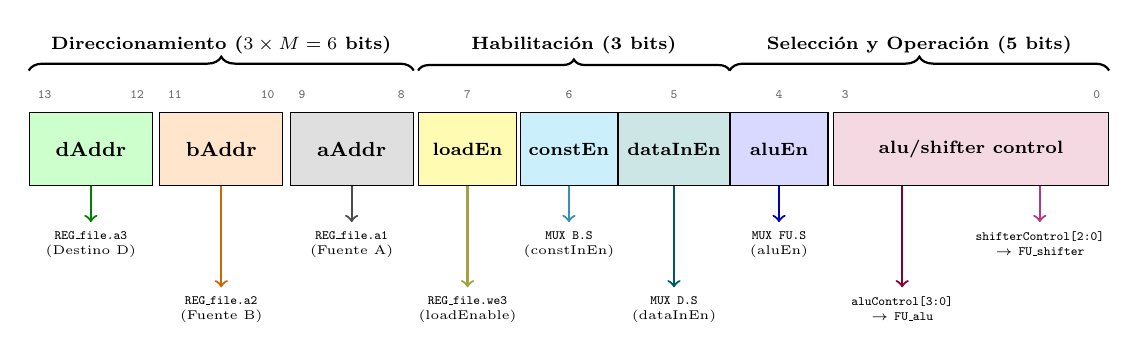
\begin{tikzpicture}[scale=0.92, transform shape,
    box/.style={draw, minimum height=1.0cm, text centered, font=\footnotesize\bfseries},
    bitnum/.style={font=\tiny\ttfamily, text=gray!80!black},
    dest/.style={font=\tiny, align=center, text=black}
  ]

  % Cajas de campos de regCTRL
  \node[box, fill=green!20, minimum width=1.7cm] (daddr) at (0.85, 0) {dAddr};
  \node[box, fill=orange!20, minimum width=1.7cm] (baddr) at (2.65, 0) {bAddr};
  \node[box, fill=gray!25, minimum width=1.7cm] (aaddr) at (4.45, 0) {aAddr};
  \node[box, fill=yellow!30, minimum width=1.35cm] (load) at (6.05, 0) {\scriptsize loadEn};
  \node[box, fill=cyan!20, minimum width=1.35cm] (const) at (7.45, 0) {\scriptsize constEn};
  \node[box, fill=teal!20, minimum width=1.45cm] (din) at (8.90, 0) {\scriptsize dataInEn};
  \node[box, fill=blue!15, minimum width=1.35cm] (aluEn) at (10.35, 0) {\scriptsize aluEn};
  \node[box, fill=purple!15, minimum width=3.8cm] (ctrl) at (13.00, 0) {\scriptsize alu/shifter control};

  % Índices de bits arriba
  \node[bitnum, anchor=south west] at ([yshift=2pt]daddr.north west) {13};
  \node[bitnum, anchor=south east] at ([yshift=2pt]daddr.north east) {12};

  \node[bitnum, anchor=south west] at ([yshift=2pt]baddr.north west) {11};
  \node[bitnum, anchor=south east] at ([yshift=2pt]baddr.north east) {10};

  \node[bitnum, anchor=south west] at ([yshift=2pt]aaddr.north west) {9};
  \node[bitnum, anchor=south east] at ([yshift=2pt]aaddr.north east) {8};

  \node[bitnum, anchor=south] at ([yshift=2pt]load.north) {7};
  \node[bitnum, anchor=south] at ([yshift=2pt]const.north) {6};
  \node[bitnum, anchor=south] at ([yshift=2pt]din.north) {5};
  \node[bitnum, anchor=south] at ([yshift=2pt]aluEn.north) {4};

  \node[bitnum, anchor=south west] at ([yshift=2pt]ctrl.north west) {3};
  \node[bitnum, anchor=south east] at ([yshift=2pt]ctrl.north east) {0};

  % Flechas y destinos abajo - Alternadas limpiamente
  \draw[->, thick, green!50!black] (daddr.south) -- ++(0,-0.5)
    node[below, dest] {\texttt{REG\_file.a3}\\(Destino D)};
  \draw[->, thick, orange!80!black] (baddr.south) -- ++(0,-1.4)
    node[below, dest] {\texttt{REG\_file.a2}\\(Fuente B)};
  \draw[->, thick, black!70] (aaddr.south) -- ++(0,-0.5)
    node[below, dest] {\texttt{REG\_file.a1}\\(Fuente A)};

  \draw[->, thick, yellow!60!black] (load.south) -- ++(0,-1.4)
    node[below, dest] {\texttt{REG\_file.we3}\\(loadEnable)};
  \draw[->, thick, cyan!70!black] (const.south) -- ++(0,-0.5)
    node[below, dest] {\texttt{MUX B.S}\\(constInEn)};
  \draw[->, thick, teal!70!black] (din.south) -- ++(0,-1.4)
    node[below, dest] {\texttt{MUX D.S}\\(dataInEn)};
  \draw[->, thick, blue!70!black] (aluEn.south) -- ++(0,-0.5)
    node[below, dest] {\texttt{MUX FU.S}\\(aluEn)};

  \draw[->, thick, purple!70!black] ([xshift=-0.95cm]ctrl.south) -- ++(0,-1.4)
    node[below, dest] {\texttt{aluControl[3:0]}\\$\rightarrow$ \texttt{FU\_alu}};
  \draw[->, thick, magenta!70!black] ([xshift=0.95cm]ctrl.south) -- ++(0,-0.5)
    node[below, dest] {\texttt{shifterControl[2:0]}\\$\rightarrow$ \texttt{FU\_shifter}};

  % Llaves superiores agrupadoras
  \draw[decorate, decoration={brace, amplitude=5pt, raise=14pt}, thick]
    (daddr.west |- 0,0.55) -- (aaddr.east |- 0,0.55)
    node[midway, above=18pt, font=\scriptsize\bfseries] {Direccionamiento ($3\times M = 6$ bits)};

  \draw[decorate, decoration={brace, amplitude=4pt, raise=14pt}, thick]
    (load.west |- 0,0.55) -- (din.east |- 0,0.55)
    node[midway, above=18pt, font=\scriptsize\bfseries] {Habilitación (3 bits)};

  \draw[decorate, decoration={brace, amplitude=5pt, raise=14pt}, thick]
    (aluEn.west |- 0,0.55) -- (ctrl.east |- 0,0.55)
    node[midway, above=18pt, font=\scriptsize\bfseries] {Selección y Operación (5 bits)};

\end{tikzpicture}
